In this section we will go through which design considerations we had when making the game.\\

\subsection{Game Features}
The game prototype we created has the following features:

\begin{enumerate}
	\item iOS Mobile Application
	\item Text story
	\item Events with player choice
	\item Event and character pictures with simple animations and sounds
	\item Map, where you can select where to go (Only on place to choose from in the prototype)
	\item Battle system where dogs battle eachother
	\item Ability to train dogs
	\item Ability to catch dogs (Will never succeed in the prototype)
	\item Option to breed dogs (Will never succeed in the prototype)
\end{enumerate}

\begin{figure}[h!] 
	\centering
    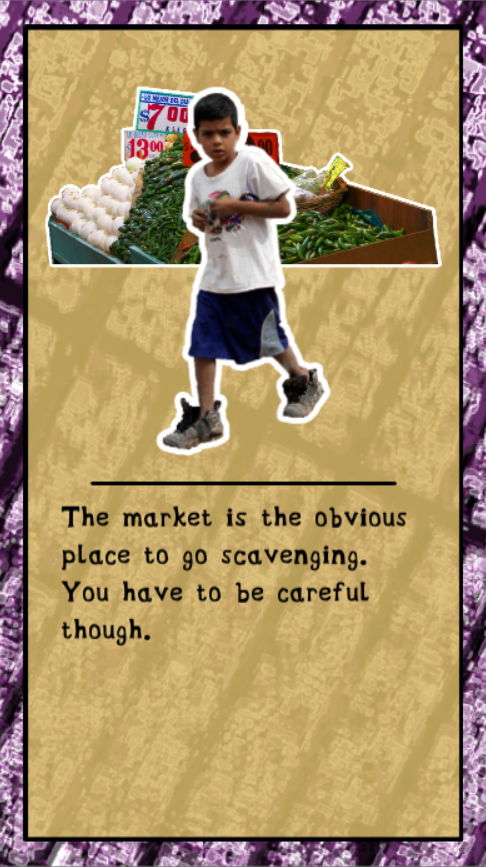
\includegraphics[width=0.5\textwidth]{GameScreen1.png}
    \caption{Story screen from the \textit{Rat Kid Dog Fight} prototype}
    \label{fig:GameScreen}
\end{figure}

%why did we choose which features?



\commenting{Choosing a vertical display for the phone for accessibility and to signal the briefness of the play session. insert this somewhere}


\subsection{Covering Prototype Limitations}
\label{limitations}
While we were creating a limited and deterministic prototype, we made several considerations, to hide the procedural and deterministic nature of the prototype. These include the map system, the ability to catch and breed, which all speak to a bigger game than the prototype is. The reason for doing this was to create an illusion of a longer game, and a potentially longer relationship with the dog. We feared that if the player knew the scale of the prototype or the already determined outcomes, they would not allow themselves to become emotionally attached to the dog. \\

To create this illusion the UI is not build for simply supporting the features of the prototype, but also to support the affordances a longer and less procedural game could include. The option to 'Breed' the dogs is a feature that is not actually included in the prototype, but since the player is forced to only catch dogs of one specific gender, they will never discover this.\\

\subsection{Lack of Player Agency in Fights}
As mentioned in \ref{Agency} we have implemented impotent options in the dog fights, which aims to create the illusion of agency. These options mimic the \textit{Pokémon} games, as seen in figure \ref{fig:PokeBattle} and \ref{fig:DogFightBattle}. 

\begin{figure}[h!] 
	\centering
    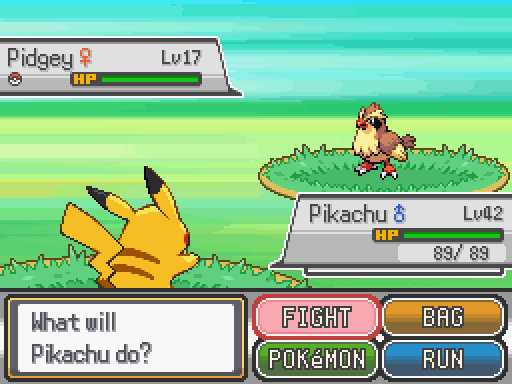
\includegraphics[width=0.5\textwidth]{PokemonBattle.png}
    \caption{A \textit{Pokémon} battle}
    \label{fig:PokeBattle}
\end{figure}

\begin{figure}[h!]
	\centering
    \includegraphics[width=0.5\textwidth]{battle.png}
    \caption{A \textit{Rat Kid Dog Fight!} battle}
    \label{fig:DogFightBattle}
\end{figure}

All these battle options does not have any effect on the actual battle. The \textit{Fight} option let the player select between \textit{Throat Bite}, \textit{Tackle}, \textit{Scratch} and \textit{Lock Bite}. While \textit{Scratch} and \textit{Tackle} are typical generic \textit{Pokémon} moves, the other two also resemble names of moves \textit{Pokémon}, with a dog fight appropiate connotation, which also makes them appear more visceral and brutal. When chosen, all of these fight-options simply give the text feedback of your character shouting something appropiate, like "Go for the throat, DOGNAME!" for selecting \textit{Throat Bite}, which also is a mediation of the television series \textit{Pokémon: The Series} (1997), where the main character, \textit{Ash}, could shout "Pikachu, use Thunderbolt!". This reference further creates the expectance of an actual effect on gameplay, since those familiar with the show, would know that there is always a direct link between what the Pokémon trainer shouts and what the Pokémon does and would expect the same causality here.
The option \textit{item} simply states that the player has no items to use and then progresses the battle. Likewise, the option \textit{Dog} states that the player "... cannot change dogs during this fight.". Similar to the (lacking) features mentioned in \ref{limitations}, this gives the player an idea of a bigger game, where they might unlock these options later on.\\

The goal with creating this illusion of player agency is to create a feeling of helplessness and hopefully the realization of no agency will put them in the place of the kid. 
\commenting{ref to 'Papers, Please'}
We want to battles to be realistically random\commenting{different word} and brutal, while still giving the player the illusion of being able to change the inevitable, creating the same superstition as mentioned in \ref{Agency}.\\

\subsection{Battle System}
Even though the player has limited agency in the fight system, we still simulate the fights with a very game-like system.\\

\begin{figure}[h!]
	\centering
    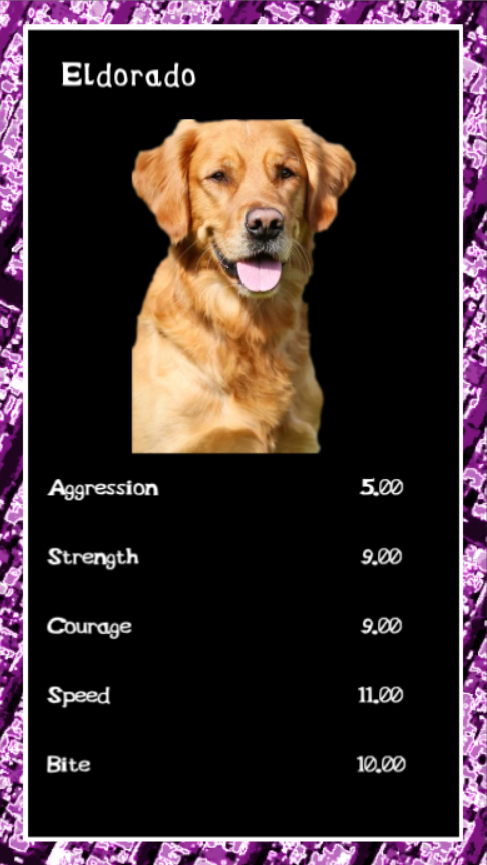
\includegraphics[width=0.5\textwidth]{DogStats.png}
    \caption{A dog stat screen from the \textit{Rat Kid Dog Fight!} prototype}
    \label{fig:DogStatScreen}
\end{figure}


The dogs has the following 5 stats: \textit{Aggression}, \textit{Strength}, \textit{Courage}, \textit{Speed} and \textit{Bite}.\\

The battle system works in the following way



%\begin{center}
	\begin{tabular}{|c|c|c|c|} 
		\hline
		Game Round & Description & Example Outcome & Feedback \\ [0.5ex] 
		\hline\hline
		Aggression Roll & Each dog has a an aggression score. The one with the highest aggression will decrease the other dogs strength speed and bite depending on the others courage rating & Dog1s 10 AGGRESSION goes against Dog2s 6 courage and decreases Dog2s STRENGTH, SPEED and BITE by 40\% & "Dog2 is intimidated by the vicious barking from Dog1" \\  
		\hline\hline
		\textit{Main loop} \\
		\hline
		Speed Roll	& The dog with the highest roll, determined by speed bites first. &	Dog1 bites first & "Dog1 snaps after Dog2s neck. \\
		\hline
		Bite roll & The biting dogs rolls BITE against STRENGTH to penetrate to kill or injur the other dog. Max roll will always penetrate, Penetrating rolls has a chance to kill or injur the other dog. Non-penetrating rolls will still have the dog bite onto and get stuck in the other dog. Low rolls will not even get stuck & Dog1 bites onto Dog2. Locking it's jaws around it. The strength of Dog2 decreases.	& "Dog1 Bites Dog2. Its jaws locking onto the skin of Dog2s stomach." \\
		\hline
		Other dogs bite Roll & Similar to above, but with penalty if the other dog has biten onto it. & "Dog2 bites Dog1. Its jaws locking onto the skin of Dog1s neck."
		\\
		\hline
	\end{tabular}
%\end{center}

\commenting{update bite roll explanation}

If a dog has its bite locked around the other one ...

If the jaws of both dogs are locked onto eachother
which simulate real dog fighting.

The main loop continues untill one of the dogs has 0 \textit{Strength}, after which the dog dies

\subsection{Actions Between Fights}
By only allowing one choice per game week, we implicitly associate a cost with the action, and an investment in your dog. In \cite{game:pokemon}

